\section{Encryption schemes}


\subsection{data layers for string type}

For string type, the newest version of cryptdb only support two onions: DET and OPE. Search was removed. Also, since the onion search has only one layer and it's quit easy to do analysis, we focus on the other two layers
in this section. For onion DET, the DET layers uses 128bits AEC-CMC encryption, which is a simple wrapper function of AES-CBC. AES-CBC will pad the plaintext if the size of plaintext can not be divided by the block size. For simplicity, in the current inplementation, if the input can be diveded by the block size, the size of the datatype is expanded by one block size. So, as we add more layers to the onion, the size of the datatype keeps increasing. 

For OPE-str, the data type will be transformed to 64 bits integer. Therefore, the characteristic of OPE-str is constrained to 64bits. The for the RND layer, blowfish will be used since the data type is transformed to integer. OPE is used only for comparing and sinced it loses information, we can not decrypt ope-str. So this onion is not suitable for backup. 

Figure 3.2 provides illustration of the onions. 



\subsection{data layers for integer}

For integer type, cryptdb create three onion: DET, OPE, and HOM. Figure 3.1 shows the layout of the onions. Hom expand any type of integer to 2048 bits binarychar. For DET and OPE, the type conversion is more complex. DET layer uses blowfish encryption, which requires 64bits integer. RND for integer also uses blowfish encryption. So for DET onion, any integer will be at most expanded to 64 bits long. For onion OPE, the first layer requires that the size of cipher text is twice the size of plaintext. If the size of ciphertext is larger than 64bits thus unable to fit into an integer type, varbinary is used instead. 



\subsection{data layout and structure}

In this section, we talk about the onion layout and How an original table is expanded whith a specific onionlayout. Since the only two data type supported for encryption, we will use and imginery table with those two data types. 



\begin{figure}[tb]
\centering
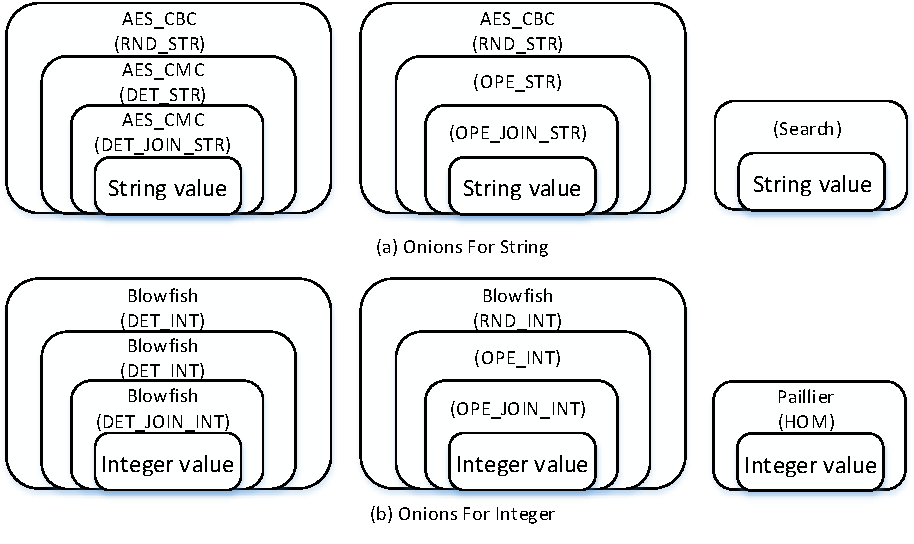
\includegraphics[width=8cm]{images/Onions.pdf}
\caption{Onion encryption layers for integer type}
\label{fig:stack3}
\end{figure}


\section{database backup methods and deduplication}

Data backup is an important functionality of database systems. All the popular database systems have backup methods. Based on how the backup is stored, we can can have two categorities of backup methods: logical backup and physical backup. Backup tools focus on low storage overhead and fast recovery. Since we do experiment with MySQL, this section focus on backup methods for MySQL. Other systems will be similar. We use backup to deal with disasters. In this section, we introduce popular backup methods. Typical backup methods also provide functions like encryption for security and compression for saving disk space.GPG tools is used for encryption.



\subsection{logical backup}

Logical backup save information in the form of SQL queries \citep{mysqlbackupdocumentatio}. For Logical backup, it's easy to control the backup granularity, and it's highly portable since the backup is in text format. MySQLdump and MySQLdumper\citep{mysqldumpper} are examples of Logical backup tools. We can also use SELECT .. INTO OUTFILE to create delimited-text files for logical backup. The basic process of logical backup is first to use select queries to pull data from the MySQL-server, and then use the data to construct Insert queries and save them into a text file. Also, Create table queries will be saved into files for recovery. We can also categorize backup method by other creterions, since we can about storage size and the logical deduplcation, we only discuss two types of backup here.





Here we describe a typical logical backup command.


\begin{itemize}
\item[--] mkdir /backups/mysqldump
\item[--] mysqldump --single-transaction --all-databases |gzip > /backups/mysqldump/today.sql.gz 
\end{itemize}






                                                 

As we can see, we can create a directory and use simple mysqldump command and options to backup our data into a file. Also, compression methods like gzip are ofthen used.

Also, If you use mydumper, you can use the following commands.

\begin{itemize}
\item[--] mkdir -p /backups/mydumper/today
\item[--] mydumper --outputdir=/backups/mydumper/today --host=localhost --compress --kill-long-queries --verbose=3 --build-empty-files --triggers --events -routines 
\end{itemize}

 
To recover the data, we can just uncompress the data and executre the sql query in the .sql file. 

you can also use binlog for backup and recovery.

\begin{itemize}
\item[--] mkdir -p /backups/binlogs
\item[--] cd /backups/binlogs
\item[--] mysqlbinlog --raw --read-from-remote-server --stop-never --verify-binlog-checksum --host=192.168.56.201 --stop-never-slave-server-id=999 mysql-bin.000001
\end{itemize}


\subsection{physical backup}

Physical bakcup consists of raw copies of directories and files that store the database contents\citep{mysqlbackupdocumentation}. In fact, simple commands like cp can be used as physical backup method. Popular physical backup tools includes ibbackup and XtraBackup\citep{xtrabackup}. MySQL store data in a set of files in a directory. Typical files includes .
This type of backup is fast since they do not convert data into logical form. Since the metadata show the data in logical form, we choose to design our strategy based on logical backup. 


Here we describe a typical physical backup workflow. 

(to be added)

The recovery form physical backup is easy. Just to uncompress the backup files and then move it the the mysql directory. 


\begin{itemize}
\item[--] service mysql stop
\item[--] rm -rf /data/mysql
\item[--] cd /backups/mylvmbackup
\item[--] tar zxf <backup file>
\item[--] mv backup/mysql /data/mysql
\item[--] service mysql start
\end{itemize}


We can find that logical backup allow user to find duplicate in the database directly, so in our design, we give our design based on logical backup.

